% This is "sig-alternate.tex" V2.0 May 2012
% This file should be compiled with V2.5 of "sig-alternate.cls" May 2012
%
% This example file demonstrates the use of the 'sig-alternate.cls'
% V2.5 LaTeX2e document class file. It is for those submitting
% articles to ACM Conference Proceedings WHO DO NOT WISH TO
% STRICTLY ADHERE TO THE SIGS (PUBS-BOARD-ENDORSED) STYLE.
% The 'sig-alternate.cls' file will produce a similar-looking,
% albeit, 'tighter' paper resulting in, invariably, fewer pages.
%
% ----------------------------------------------------------------------------------------------------------------
% This .tex file (and associated .cls V2.5) produces:
%       1) The Permission Statement
%       2) The Conference (location) Info information
%       3) The Copyright Line with ACM data
%       4) NO page numbers
%
% as against the acm_proc_article-sp.cls file which
% DOES NOT produce 1) thru' 3) above.
%
% Using 'sig-alternate.cls' you have control, however, from within
% the source .tex file, over both the CopyrightYear
% (defaulted to 200X) and the ACM Copyright Data
% (defaulted to X-XXXXX-XX-X/XX/XX).
% e.g.
% \CopyrightYear{2007} will cause 2007 to appear in the copyright line.
% \crdata{0-12345-67-8/90/12} will cause 0-12345-67-8/90/12 to appear in the copyright line.
%
% ---------------------------------------------------------------------------------------------------------------
% This .tex source is an example which *does* use
% the .bib file (from which the .bbl file % is produced).
% REMEMBER HOWEVER: After having produced the .bbl file,
% and prior to final submission, you *NEED* to 'insert'
% your .bbl file into your source .tex file so as to provide
% ONE 'self-contained' source file.
%
% ================= IF YOU HAVE QUESTIONS =======================
% Questions regarding the SIGS styles, SIGS policies and
% procedures, Conferences etc. should be sent to
% Adrienne Griscti (griscti@acm.org)
%
% Technical questions _only_ to
% Gerald Murray (murray@hq.acm.org)
% ===============================================================
%
% For tracking purposes - this is V2.0 - May 2012

\documentclass{sig-alternate}

\usepackage{url}

\def\sharedaffiliation{
\end{tabular}
\begin{tabular}{c}}

\begin{document}
%
% --- Author Metadata here ---
%\conferenceinfo{WOODSTOCK}{'97 El Paso, Texas USA}
%\CopyrightYear{2007} % Allows default copyright year (20XX) to be over-ridden - IF NEED BE.
%\crdata{0-12345-67-8/90/01}  % Allows default copyright data (0-89791-88-6/97/05) to be over-ridden - IF NEED BE.
% --- End of Author Metadata ---

\title{Gang Scheduling Java Applications with Tessellation}

\numberofauthors{4}

\author{
Benjamin Le \and Jefferson Lai \and Wenxuan Cai \and John Kubiatowicz\titlenote{The Parallel Computing Laboratory, UC Berkeley, CA, USA}\\
      \sharedaffiliation
      \affaddr{\{benjaminhoanle, jefflai2, wenxuancai\}@berkeley.edu, kubitron@cs.berkeley.edu}\\
      \affaddr{Department of Electrical Engineering and Computer Science }\\
      \affaddr{University of California, Berkeley }\\
      \affaddr{Berkeley, CA 94720-1776}
}

\CopyrightYear{2014}

\maketitle
\begin{abstract}
Java Virtual Machines (JVM) are responsible for performing a number of tasks in addition to program execution, including those related to garbage collection and adaptive optimization. Given the popularity of the Java platform and the rapid growth in use of cloud computing services, cluster machines are expected to host a number of concurrently executing JVMs. Despite the virtual machine abstraction, interference can arise between JVMs and degrade performance. One approach to prevent such multi-tenancy issues is the utilization of resource-isolated containers. This paper profiles the performance of Java applications executing with the resource-isolated cells of Adaptive Resource-Centric Computing and the Tessellation OS. Within this setup, we demonstrate how overall performance and JVM efficiency for the DaCapo benchmarks and Cassandra on the Yahoo Cloud Serving Benchmark degrade. We compare the effect of gang scheduling the threads of a cell together with using a simple global credit scheduler. We show that from the limited results we observed, there is no convincing evidence of gang scheduling yielding any kind of benefit, but also that a more complete evaluation may still be needed.
\end{abstract}

% Same categories as Juan's DAC 2013 Tesselation paper
\category{D.4.1}{Operating Systems}{Process Management -- Scheduling}
\category{D.4.8}{Operating Systems}{Performance -- Measurements, Monitors}

\terms{Multicore, parallel, quality of service, resource containers}

\keywords{Adaptive resource management, performance isolation, quality of service}

\section{Introduction}
\label{sec:introduction}
The Java Virtual Machine (JVM) abstraction provides a consistent, contained execution environment for Java applications and has played a significant role in Java's popularity and success in recent years. The JVM abstraction encapsulates many tasks and responsibilities that make development faster and easier. For example, by handling the translation of portable Java bytecode to machine code specific to the lower level kernel and system architecture, the JVM allows developers to write an application once and run it in a number of different environments. While there exist a number of JVM implementations, maintained both privately and publicly, in general, implementations adhere to a single JVM specification. We refer the reader to \cite{lindholm2014java} for a complete specification, but summarize the roles of two key, highly researched components of the JVM: the garbage collector (GC) and the adaptive optimization component of the ``just in time" (JIT) compiler \cite{hotspot:whitepaper}.

Garbage collection is the process of cleaning up unused memory so that developers do not need to manage memory themselves. While this makes development easier and can drastically reduce the number of memory related bugs, garbage collectors are very complex and consumes resources, including time. Many techniques for garbage collection have been developed from simple reference counting, to parallelized stop-and-copy, to generational garbage collection \cite{lins1996garbage}. Each technique differs in how to locate ``live" objects, when to run, whether and when execution needs to be halted, what memory needs to be touched, and how objects in memory should be moved.

The JIT compiler, on the other hand, is responsible for compiling segments of bytecode into native machine instructions. Modern JIT compilers are extended with adaptive optimization techniques \cite{suganuma2001dynamic}, which attempt to optimize performance by dynamically compiling and caching these segments of code during run time. The result is a drastic performance improvement over simply interpreting the bytecode. Exactly how much compilation occurs before versus after a program begins executing and how much of a given program is interpreted varies across JVMs and significantly affects the performance characteristics of the program. While more advanced optimization results in higher performing code, as with GC techniques, it generally also requires more resources to perform, incurring higher overhead and impact on the program's performance.

Together, garbage collection and adaptive optimization require the JVM to perform many background tasks in addition to program execution. While this design works well when there is a small number of Java applications on a machine, it may not scale well when there are many Java applications running concurrently on a single machine. This type of situation can often be found on the machines in cloud computing clusters. Given the ubiquity of Java based software applications, as demand for cloud computing and hosting services increase, understanding the types of multi-tenancy issues that may arise becomes critical to progress. For example, a machine in the cloud could be asked to host multiple instances of Hadoop File System (HDFS) \cite{shvachko2010hadoop}, Hadoop MapReduce \cite{bialecki2005hadoop}, and Spark \cite{zaharia2010spark}, simultaneously, with each instance having a dedicated JVM. As all of these long-running JVMs must ultimately be multiplexed onto a single set of hardware, interference may arise between the tasks of each JVM. For certain applications, such as those with strict timing requirements or quality of service (QoS) guarantees, this interference may lead to unacceptable performance.

In addition to investigating the significance of the issues named above, we consider a potential solution made possible with the \textit{Tessellation} operating system architecture and the \textit{Adaptive Resource-Centric Computing (ARCC)} system design paradigm \cite{colmenares2010resource, colmenares2013tessellation, liu2009tessellation}. In ARCC, applications execute within stable, isolated resource containers called \textit{cells}. In addition to implementing cells, the ARCC-based Tessellation kernel uses \textit{two-level scheduling}, which decouples the allocation of resources to cells (the first level) from scheduling how these resources are used within cells (the second level). In this paper, we apply and evaluate gang scheduling \cite{feitelson1992gang} as a second level scheduling policy. In particular, we execute a single application in each cell and run multiple cells on a single, multi-core machine, gang scheduling each cell's resources together. By measuring the performance of these applications with and without gang scheduling, we show the effect of gang scheduling at mitigating interference for OpenJDK's HotSpot JVM.

The remainder of this paper is organized as follows. Section~\ref{sec:background} provides background on the HotSpot JVM and the Tesselation architecture. Section~\ref{sec:dacapo} and section~\ref{sec:cassandra} describe our experimental setup and results with two Java different benchmark suites. Section~\ref{sec:gs} describes our results when using a gang scheduler. In section~\ref{sec:relatedwork} we present a survey of related work. We discuss directions for future work in section~\ref{sec:futurework} and conclude in section~\ref{sec:conclusion}.

\section{Background} \label{sec:background}
This section provides an overview of the relevant features of OpenJDK's HotSpot JVM and of the primary features of the Tessellation manycore operating system.

\subsection{HotSpot}
There currently exist two primary implementations of the HotSpot JVM. One is owned and maintained privately by Oracle and the other is an open source version maintained alongside the OpenJDK project. Despite being separately maintained, the two implementations are strikingly similar in methodology and performance. This is largely due to the fact that each stems from the same version made public by Sun Microsystems as well as the fact that the two sets of contributors overlap considerably. The primary differences between the two stem from Oracle's addition of several non-essential, auxiliary components. As such, and for lack of detailed documentation from OpenJDK, we present two key components of the Oracle HotSpot JVM here and make the, we believe valid, assumption that our discussion applies wholly to the OpenJDK implementation.

The HotSpot JVM is designed as a high-performance environment for Java applications with a focus on performance optimization. On top of implementing the features required by the aforementioned Java Virtual Machine specification, HotSpot provides a number of options and operating modes for tuning for different use cases. This focus is embodied in HotSpot's implementation of the garbage collector and adaptive optimizer. We now summarize the main features of these two components and describe how the synchronization characteristics of each make gang scheduling an appealing option.

\subsubsection{HotSpot Garbage Collection}
The garbage collector in HotSpot is a \textit{generational garbage collector} \cite{hotspot:memory} that partitions the heap into two generations: the \textit{young generation}, the \textit{old generation}. The idea behind this is that most allocated objects have short lives and do not survive more than a small number of garbage collections. Thus, efficiency is improved by primarily allocating from the smaller young generation and collecting this frequently while holding long-living, tenured objects in the larger old generation and collecting it less frequently. These significantly differing characteristics mean that the young and old generations can, and should, be collected using different collection algorithms in the interest of performance and efficiency.

The young generation is separated into an \textit{eden space} and two \textit{survivor spaces}. Most new objects are allocated from the eden space.\footnote{Some large objects that do not fit may be allocated directly to the old generation.} When that becomes full a \textit{minor collection} occurs, which collects space from dead objects and moves them between the survivor spaces. At the end of the collection the only one survivor space contains active data. These are the live objects that survived collection but have not been promoted to the old generation.\footnote{If not enough space exists in the to space, the remaining objects are moved to the old generation.} HotSpot allows this collection to be performed serially or in parallel. While the serial version may be applicable for small scale, personal uses, we focus on the the parallel version, which is more appropriate and the default for the server class machines we are interested in. In both cases, minor collections are always \textit{stop-the-world} collections that require application execution to be paused. As such, in the case of parallel collection, a natural barrier is created at both the start and end of a minor collection, and a small amount of communication between threads is required to initially divide the work among threads.

In contrast to the young generation, the old generation is not further divided; the entire space is used to hold objects that are large or long-living. When the old generation becomes full, a \textit{major collection} occurs, during which both generations are collected, with the young generation collection typically occurring first. The collection of the old generation can be serial or in parallel and done in a stop-the-world fashion or concurrently during application execution. Again, while a serial \textit{mark-sweep-compact} algorithm is available, we focus on two parallel algorithms which utilize multiple cores and reduce pause times.

The \textit{parallel compacting (PC)} collector is a stop-the-world collector that collects the old generation in three phases. In the \textit{mark} phase, a set of ``root" objects are divided among threads and live objects are marked, along with metadata for the region containing them. The \textit{summary} phase is performed serially and calculates the density of live data for each region so that the following parallel \textit{compaction} phase can move and compact the data. Utilizing parallelism helps reduce pause times, especially when the size of the old generation is large. However, in some cases, even this reduced pause time is still too long. For such situations, HotSpot provides the \textit{concurrent mark-sweep (CMS)} collector. Unlike the PC collector, the CMS collector only requires a small number of short pauses at certain synchronization points. CMS collection begins by a short pause that identifies an initial set of root objects. After this pause, the application resumes execution while a single GC thread identifies the live objects reachable by the root objects in the \textit{concurrent mark} phase. Because the application is running during this phase, a second pause is made and multiple threads are used to find live objects that were missed. Afterwards, the application can resume while a single thread reclaims the garbage space in the \textit{concurrent sweep} phase. The CMS collector helps avoid long pauses, but since it does not perform compaction, allocations and minor collections may take longer. This trade-off can be favorable for applications with short pause time requirements. Both the PC collector and the CMS collector have synchronization points or barriers between each of their respective phases. In HotSpot, per-thread jobs are implemented so that they are largely independent and thus, a minimal amount of synchronization is required within phases.

\subsubsection{HotSpot Adaptive Optimization}
Traditional JIT compilers perform compilation just before execution, and thus are limited in terms of compile time and the types of optimizations they make. For example, since Java supports features such as dynamic class loading, it cannot perform some types of aggressive optimizations such as extensive method-inlining. HotSpot's adaptive optimization component addresses several of these obstacles by initially interpreting the entire program and selectively compiling only certain parts of the code during run time \cite{hotspot:whitepaper}. This technique is based on the observation that for many programs, most of program's execution time is spent executing only a small portion of the program's code. Instead of spending valuable time and resources compiling code which is rarely executed, the compiler can detect ``hot spots" in the code that are run very frequently and focus optimization on those parts. This includes, but is not limited to, compiling and caching these ``hot spots." In addition, by \textit{code profiling} or monitoring and gathering information about the program's execution patterns, HotSpot can perform some of the aggressive optimizations done by static compilers, including method-inlining, as well as new types of optimization techniques. One important example of this is \textit{dynamic deoptimization}. Since execution patterns can change and new code can be loaded while the program is running, the HotSpot advanced optimizer can deoptimize (e.g. revert back to interpretation) and reoptimize the code in response.

Of course, performing this profiling, analysis, optimization consumes resources. Profiling itself actually incurs a relatively small amount of overhead. It consists largely of maintaining performance counters to monitor method and loop entries \cite{hohensee:overview}. However, the analysis and JIT compilation portion of the optimizer can consume a significant amount of resources, depending on how the program is written and how stable the code profile is. This compilation and analysis is performed alongside the application. In addition, a fair amount of synchronization is required in order to dynamically modify code paths safely and efficiently.

HotSpot comes packaged with three choices for compilers: the client compiler, server compiler, and tiered compiler. The client compiler focuses on being fast and minimizing startup delays by performing mostly quick and simple local optimizations. In contrast, the server compiler is designed for server-like, long-running programs. It performs a number of complex, advanced optimizations that require extra time in order to gather the large amount of profiling data needed. The tiered compiler attempts to achieve ``the best of both worlds" by initially using a client compiler to compile profiled code quickly. The client compiler ultimately feeds into a server compiler, which can use the compiled, profiled code to perform more advanced optimizations quickly. In this paper, we utilize the server compiler because we expect multi-tenant JVM issues to be more prevalent when the JVMs host long-running tasks. We choose the server compiler over a tiered compiler simply because it is much more widely used than the tiered compiler, which is relatively new.

\subsection{Tessellation}
\textit{Adaptive Resource Centric Computing (ARCC)} is a design paradigm which establishes an interface between resources and applications through the abstraction of \textit{cells} \cite{colmenares2013tessellation}. A cell is essentially a stable, consistent resource container for applications. A cell can also be used as a wrapper for a set of resources and exposes a service interface for that resource to other cells. Resources are allocated to cells and the applications running within them are provided quality of service guarantees for those resources. Within ARCC, resource allocations to cells are automatically adjusted in such a way to best meet application requirements.

The Tessellation OS architecture \cite{colmenares2010resource, colmenares2013tessellation, liu2009tessellation} implements cells using an approach called \textit{space-time partitioning}, in which hardware resources are virtualized, ``spacially" partitioned, and time multiplexed. Concretely, this means that resources such as CPU cores, memory, and service guarantees from other cells can be partitioned and shared by a number of processes. Tessellation's model for accomplishing this is through \textit{two-level scheduling}, which separates resource allocation (first level) from how those resources are used (second level).

The cell abstraction offered by the ARCC and Tessellation align very well with the goals of the JVM abstraction. Perhaps most importantly, both models attempt to provide a stable and isolated execution environment for applications so they do not need to concern themselves with lower level system complexities. Moreover, the QoS guarantees, resource isolation and freedom of scheduling within cells in Tessellation are able to provide conditions near that of a dedicated machine. In the rest of this paper, we profile the effect of multiple, concurrent JVMs on the performance of applications with different types of workloads when running on an implementation of the Tessellation OS. We investigate the significance of inter-JVM interference and the cost of preventing it by comparing the effectiveness of gang scheduling the resources within a cell (i.e. the resources provisioned to a given JVM) with using a simple global credit-scheduler \cite{ackaouy2006xen}.

\section{Dacapo with Xen} \label{sec:dacapo}
The DaCapo benchmark suite is a diverse set of open source, real world applications \cite{blackburn2006dacapo}. The applications in the suite were chosen to maximize coverage of the types of applications run in the wild and to be relatively easy to use and measure. These applications are also well known to put considerable pressure on the JVM garbage collector and to improve significantly from JVM warm up. The benchmark harness supports multiple workload sizes, configurable number of iterations to run a benchmark, and the reporting of a performance stable iteration.

We utilize the DaCapo 9.12 bach benchmark suite released in 2009. Only a subset of this suite is used for our experiments (avrora, jython, luindex, xalan). The subset was chosen based off which benchmarks ran without errors within our guest OS, OS$^{v}$ \cite{aviOSv2014}. The characteristics of these benchmarks are listed below.
\\\\
\textbf{Avrora:} Avrora is a multithreaded application which simulates programs being run on a grid of AVR microcontrollers. Each microcontroller is simulated by a single thread. Avrora exhibits high fine-grained synchronization between simulator threads.
\\\\
\textbf{Jython:} Jython is a Python interpreter written in Java which runs the \textit{pybench} benchmark. The bulk of the tests in \textit{pybench} are single-threaded. For those few tests that are multithreaded, a thread is created for each available CPU. 
\\\\
\textbf{Luindex:} Luindex is a text indexing tool that indexes the works of Shakespeare and the King James Bible. Although some helper threads are forked internally, luindex is primarily driven by a single thread.
\\\\
\textbf{Xalan:} Xalan transforms a XML document featuring the works of Shakespeare into HTML. Xalan is multithreaded, creating a thread for each available CPU. Threads process elements off a work queue in parallel.

\subsection{Experimental Setup}\label{subsec:expsetup}
\begin{figure}
\centering
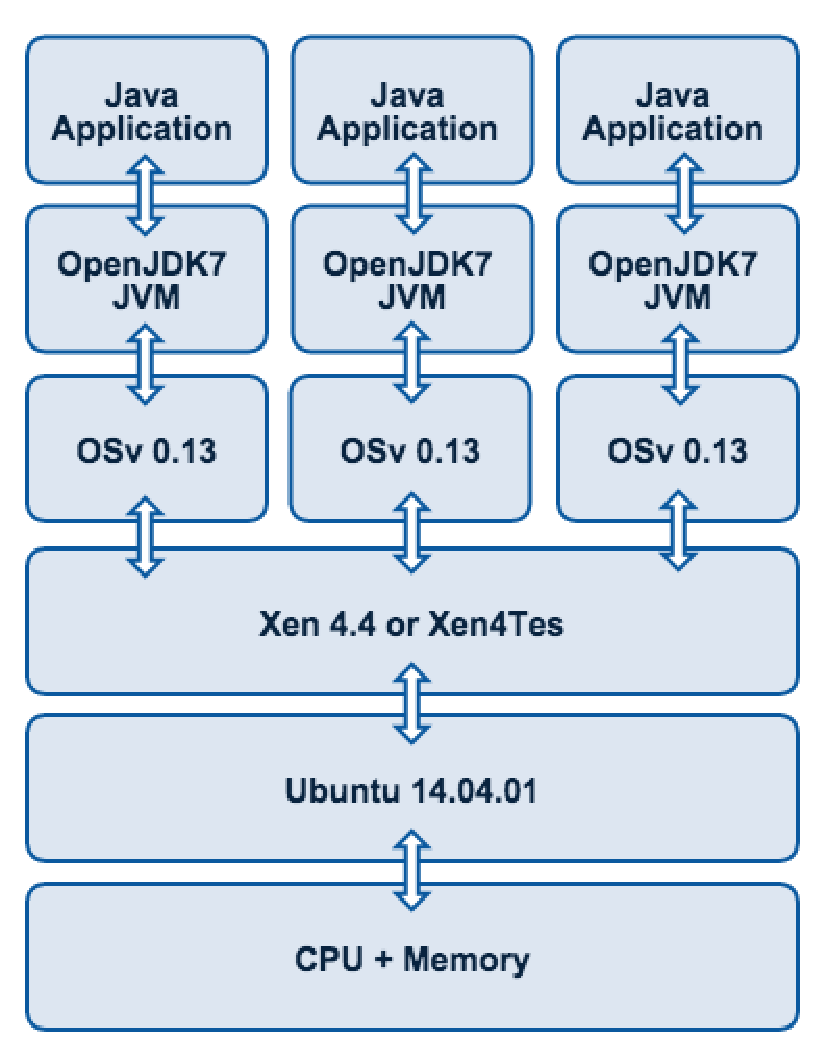
\epsfig{file=figures/dacaposetupdiagramcrop.eps, height=3.75in, width=3in}
\caption{The application layering of our experimental setup.}
\label{fig:dacaposetup}
\end{figure}

Figure~\ref{fig:dacaposetup} showcases our experimental setup. Our setup uses the OpenJDK7 implementation of the Java platform. We deploy our JVMs in Virtual Machines running the OS$^{v}$ 0.13 Operating System \cite{aviOSv2014}. OS$^{v}$ VMs are run as guest domains on the Xen 4.4 hypervisor \cite{barham2003xen}. The hypervisor runs on a 2-socket machine with 2 Intel Core i7-920 processors at 2.67GHz (4 cores per socket, Hyperthreading off,  8 total CPUs).  Our test machine has 12GB of physical memory and runs Ubuntu 14.04.01. Each Xen guest domain runs with 6 vCPUs and is allocated 512MB of memory. We run Xen domains within a 6-CPU Pool while reserving 2 CPUs and 3GB of memory for Domain-0.  

We run three experiments using DaCapo and Xen's default credit scheduler for CPU resources. First, we measure the overall performance of running JVMs in parallel. Second, we measure the pause times of a \textit{stop-the-world} parallel garbage collector. Third, we explore the performance of HotSpot's adaptive optimizer during the warm up phase while running along side multiple JVMs. For all experiments, the same benchmark is run across all concurrent JVMs using the default workload size.

\subsubsection{Overall Performance} \label{sssec:overallperf}
For each benchmark in our subset, we run 1, 2, 4, 8, and 16 JVMs in parallel, with maximum heap sizes of 64MB, 128MB, and 256MB. We warm up our JVMs by running the benchmark for some number of iterations. The number of warm up iterations is empirically determined by calculating the average number of iterations needed until performance stabilizes for that benchmark. We continue to run the benchmark until all JVMs complete at least 5 more iterations after warm up.  The execution times of these 5 iterations are recorded. We also recorded the percentage of CPU time each domain spends in the \textit{concurrency hazard} run state using the xentrace and xenalyze tools. Concurrency hazard is the domain state where some vCPUs are running while the other vCPUs are waiting to be scheduled to run. 

\subsubsection{Parallel Garbage Collector Performance}
In the same setup as Experiment 1, we run the parallel JVMs with the \textit{-XX:-UseParallelOldGC} flag turned on. This specifies that a parallel garbage collector be used for both the young and old generations. We record the GC pause times for both minor and major(full) collections that occur during the execution of the next 5 iterations after warm up.

\subsubsection{Adaptive Optimizer Performance}
First, for each benchmark, we run a single JVM in isolation with maximum heap sizes of 64MB, 128MB, and 256MB. Similarly to Experiment 1, we record the execution times of the next 5 iterations after warm up. Next, we warm up a single JVM with the same heap sizes while the machine is under the load of 15 other JVMs running the same benchmark. After warm up, we kill the other JVMs and run the single JVM in isolation; again recording the execution times of the next 5 iterations. We repeat these steps for each combination of benchmark and heap size 5 times recording 5 data points per combination.

\subsection{Results}
In the interest of space, we only showcase results for two of our benchmarks, avrora and xalan. The other two benchmarks exhibit results that a similar to and more pronounced in avrora and xalan.

\subsubsection{Overall Performance} \label{sssec:overallperfresults}
We begin by profiling overall performance as we scale the number of concurrently running JVMs on our system. The left-most column in Figure~\ref{fig:overallperf} shows the overall total run time slowdown relative to 1 JVM. We calculate slowdown by dividing the mean total run time for the next 5 iterations after warm up for N JVMs over that for 1 JVM. For avrora and xalan respectively, performance is stable for up to 4 and 2 concurrently running JVMs. Because these benchmarks are quite old, \textit{resource saturation} does not occur until multiple JVMs are deployed. After saturation, there is a roughly linear increase in slowdown.

In the center column, we graph the average fraction of CPU time spent in the concurrency hazard run state as we scale up the number of JVMs. We wish to explore whether the credit scheduler is naturally scheduling the vCPUs for our applications together, or in other words, imitating gang scheduling. We are most interested in the concurrency hazard run state because this is when vCPU clock skew occurs, something that can be reduced if vCPUs are gang scheduled together. We hypothesize that increasing the number of JVMs will increase the chance of being in the concurrency hazard run state. Our results show that if this is true, the fraction time spent in concurrency hazard spikes and then slowly dips off scaling to 16 JVMs. After investigating why this dip off occurs, we discovered that domains spend a majority of their time in the partial contention run state at 16 JVMS, up to 50\% for avrora and 60\% for xalan. Partial contention is when some vCPUs are waiting to be run while others are blocked, as opposed to running for concurrency hazard. We believe that the increase in time spent in partial contention is due to hitting IO bounds when scaling up the number of JVMs.

In the right most column, we graph the continous density function for iteration run times of all 5 iterations after warm up across all JVMs. We are interested in how variation for run time is affected as we scale up the number of JVMs. We only show CDFs for 128MB maxmium heap size because CDFs for 64MB and 256MB are very similar. For both avrora and xalan, we observe longer tails on both ends when running 16 JVMs in parallel. This indicates that the end user running these JVMs will experience more inconsistent performance under increasing multi-tenancy in the system. 

Under gang scheduling, we do not expect overall performance to improve but we do believe that performance can be \textit{more consistent} due to a more accurate abstraction of CPU resources.

\begin{figure*}
\centering
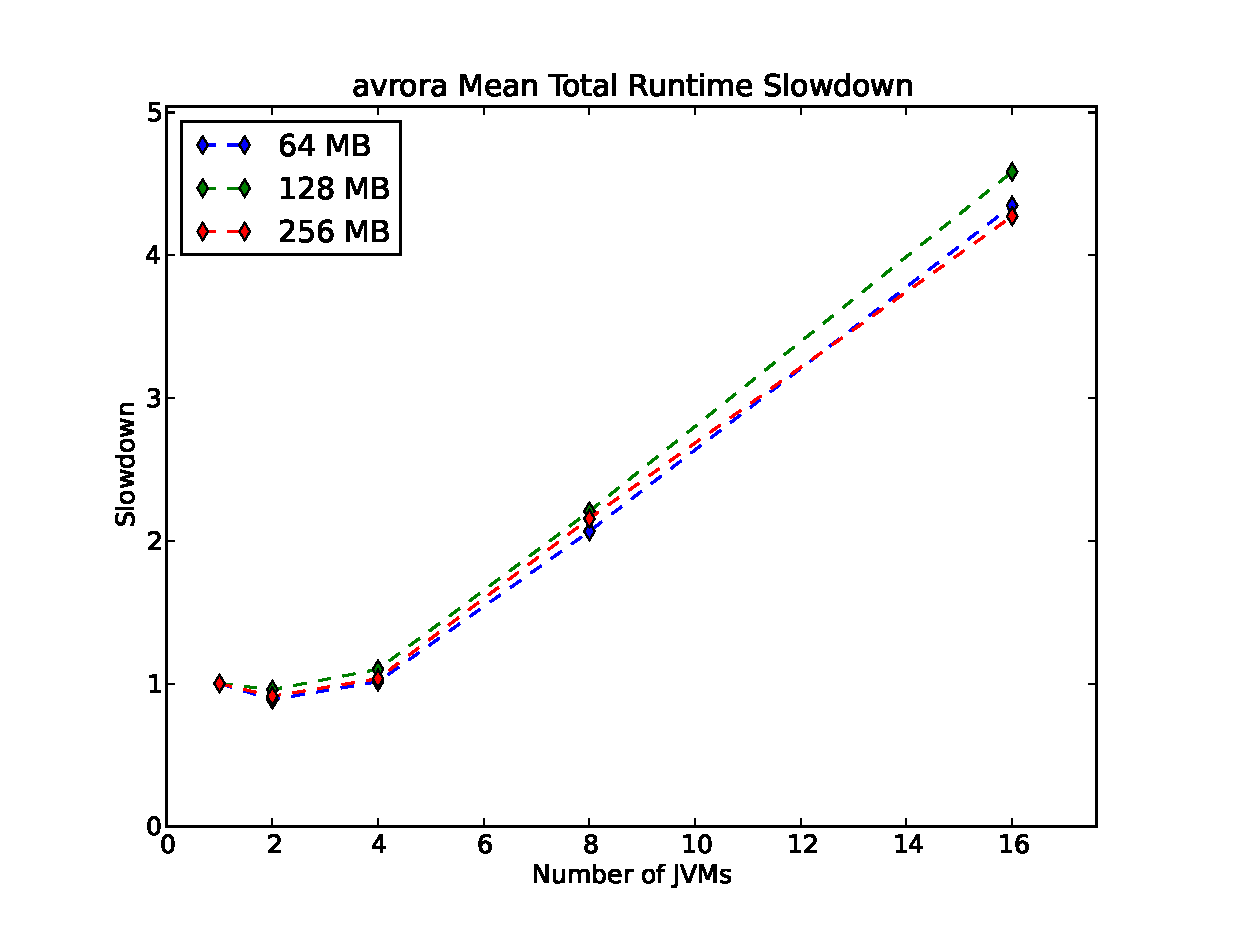
\epsfig{file=figures/slowdowns/avrora.eps,  height=1.5in, width=2.25in}
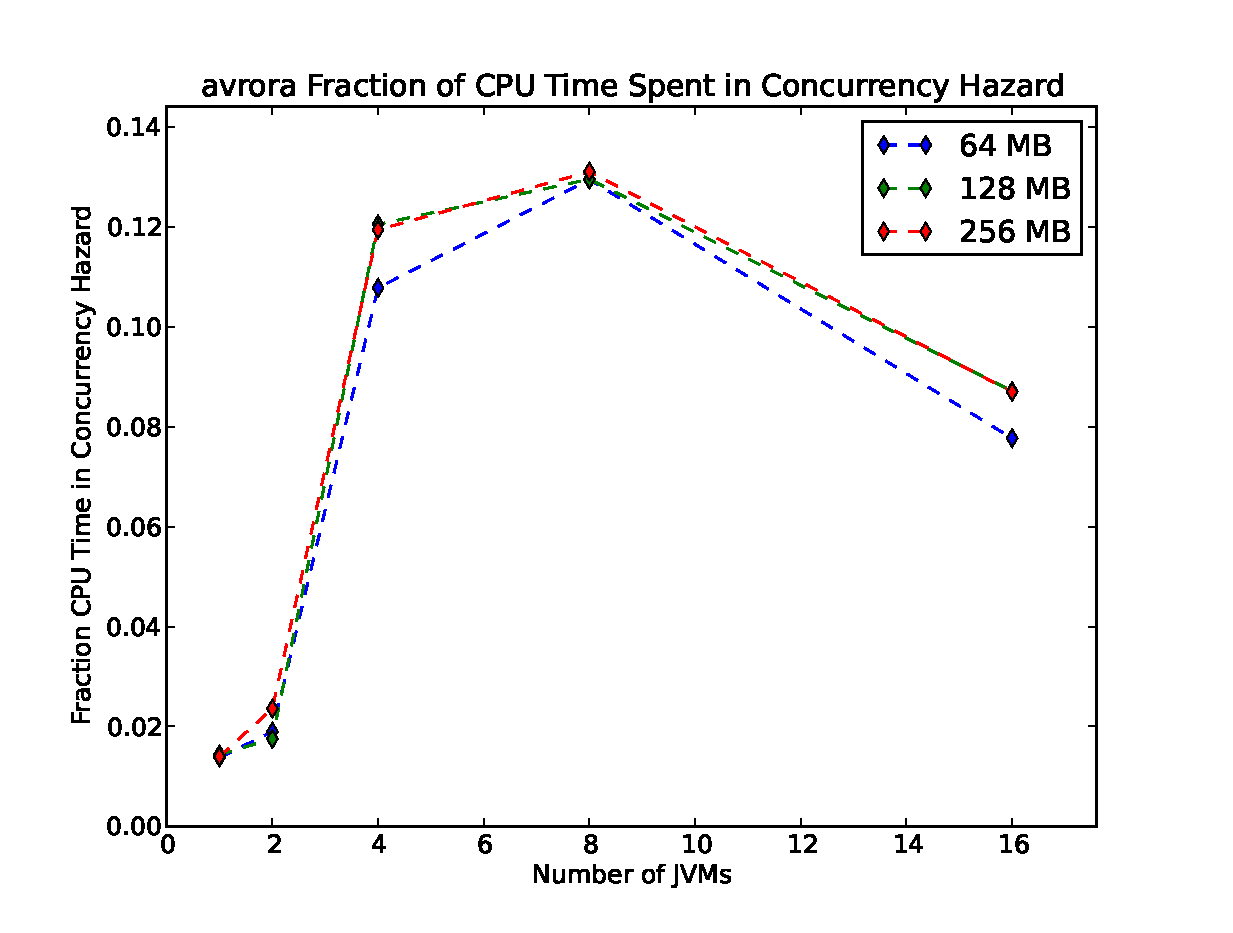
\epsfig{file=figures/xenalyze/avrora.eps,  height=1.5in, width=2.25in}
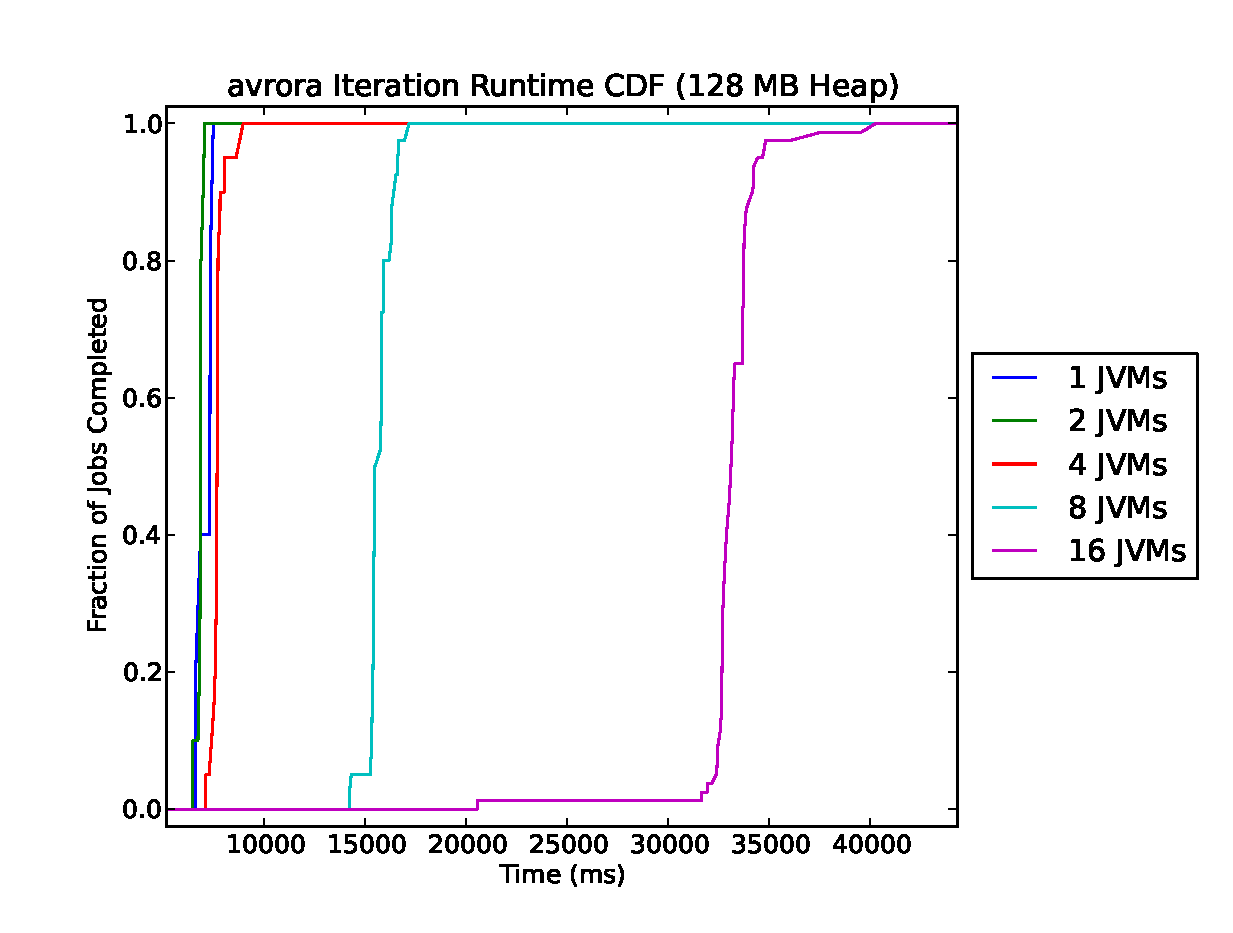
\epsfig{file=figures/cdfs/avrora_128MB.eps,  height=1.5in, width=2.25in}
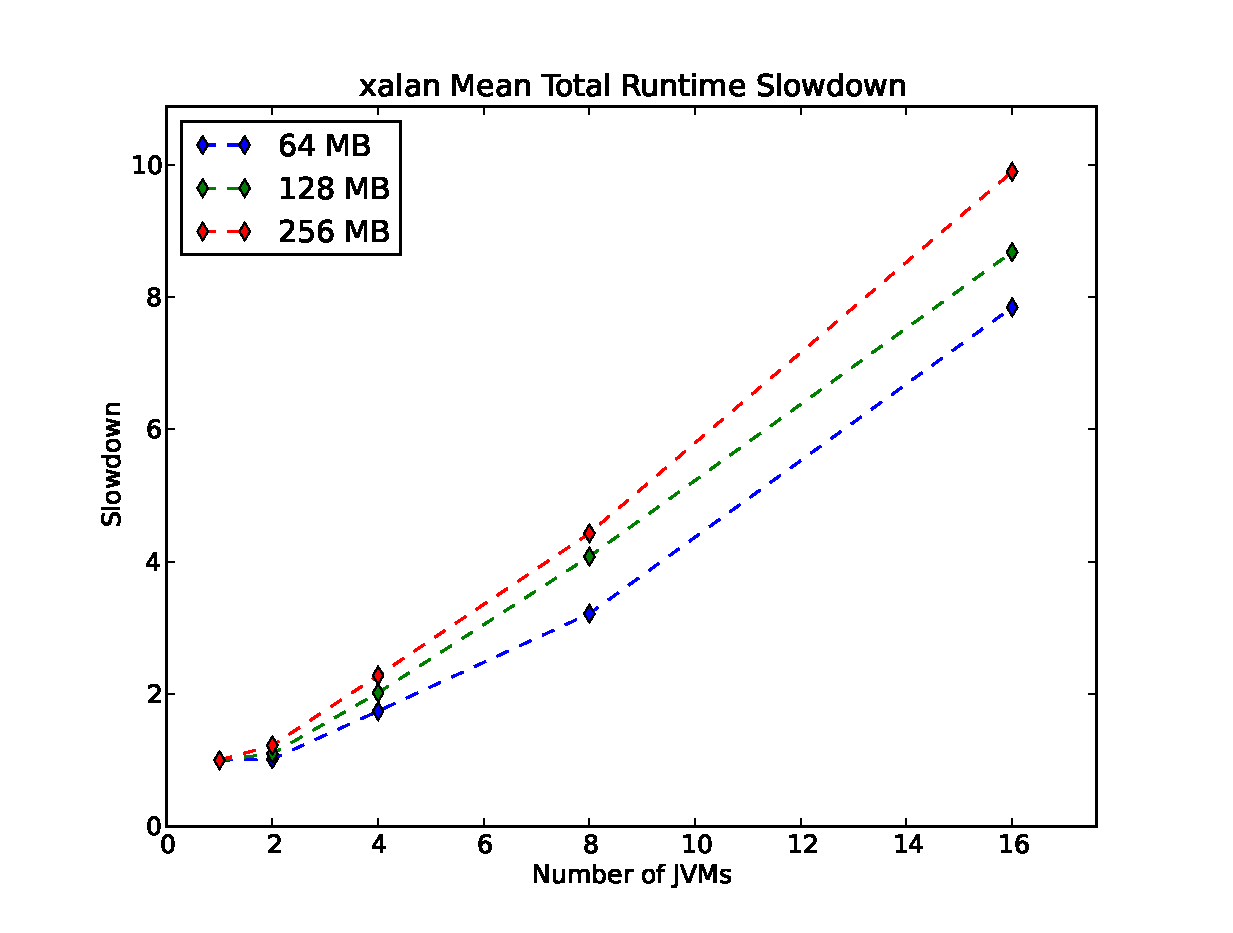
\epsfig{file=figures/slowdowns/xalan.eps, height=1.5in, width=2.25in}
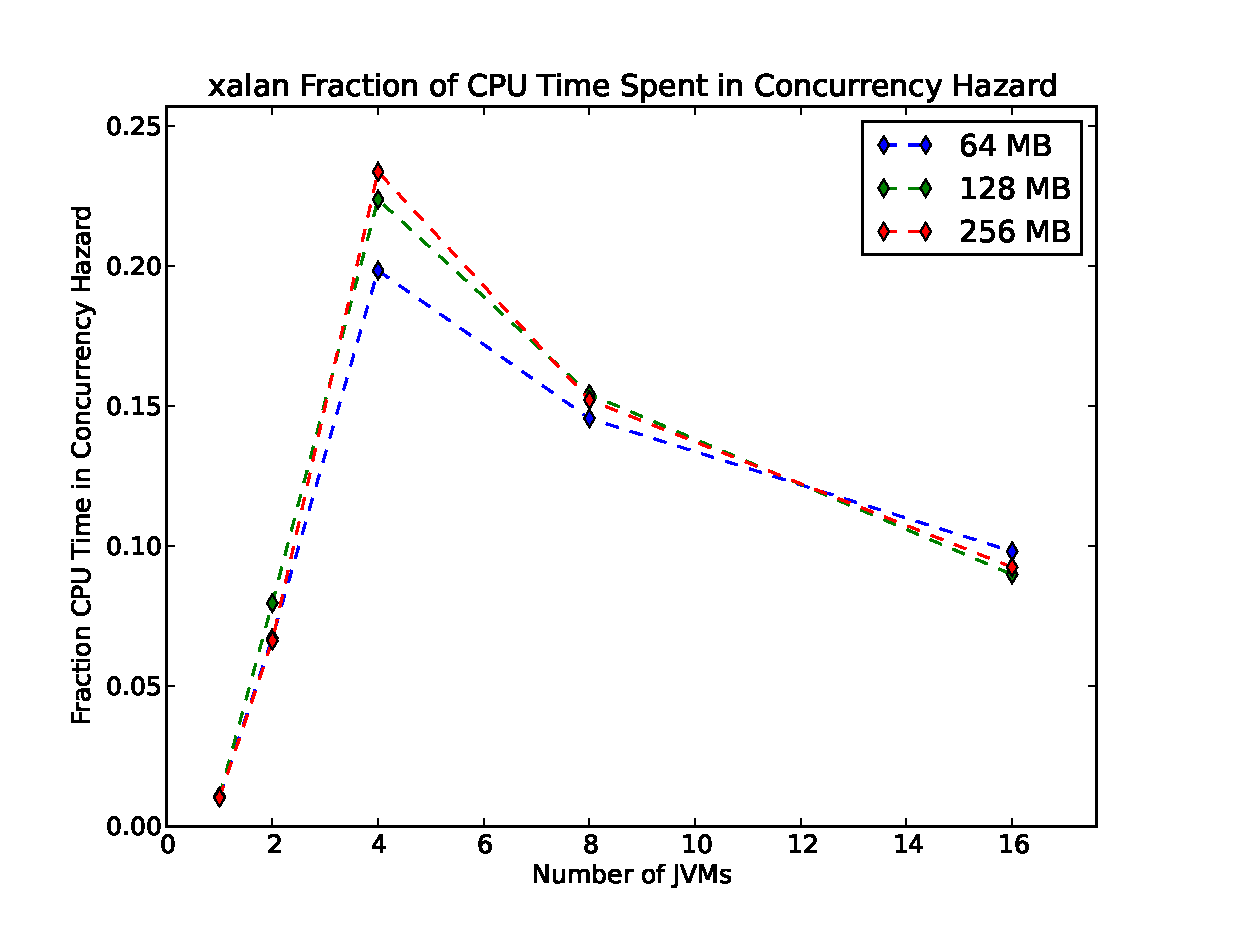
\epsfig{file=figures/xenalyze/xalan.eps,  height=1.5in, width=2.25in}
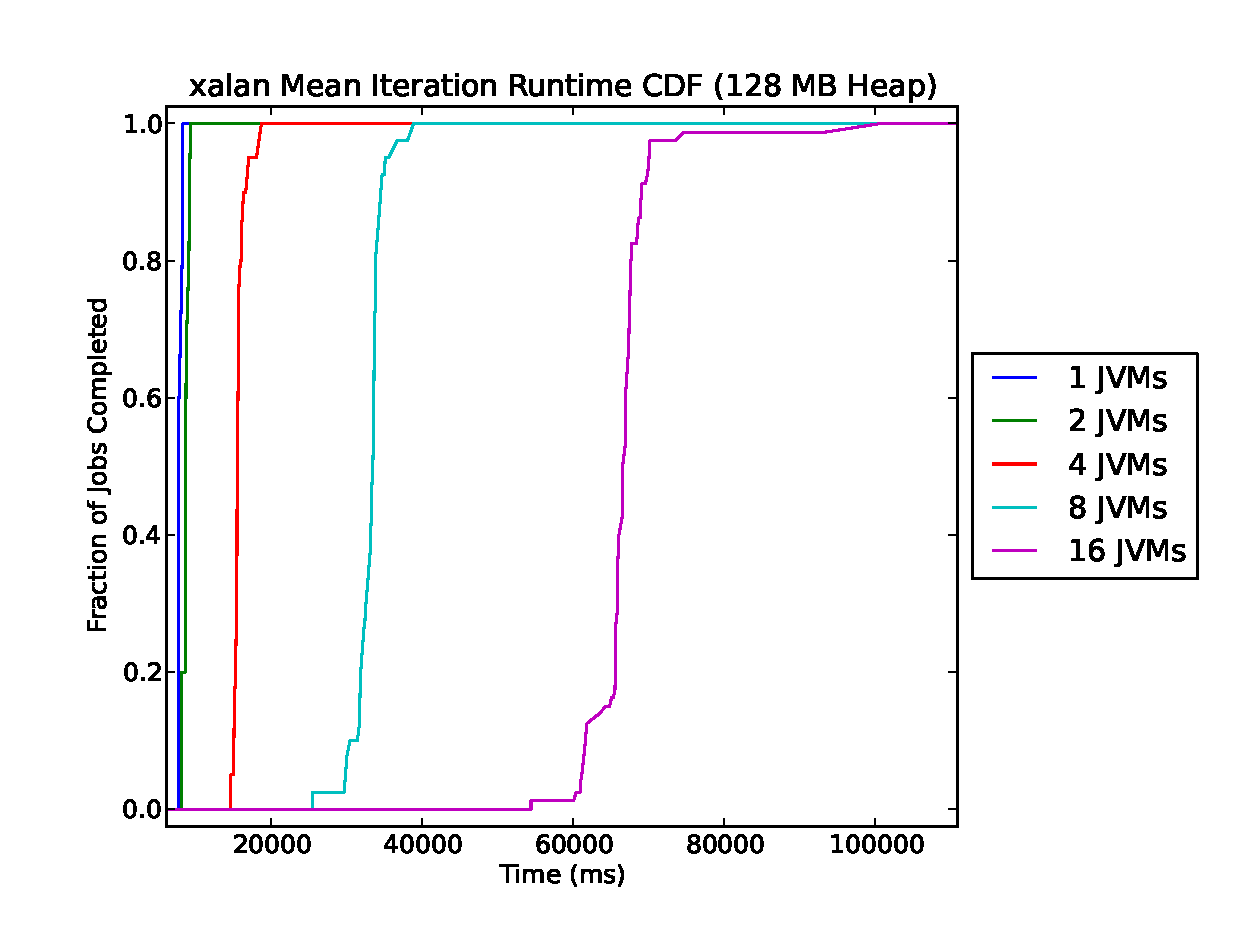
\epsfig{file=figures/cdfs/xalan_128MB.eps,  height=1.5in, width=2.25in}
\caption{Run time slowdown relative to 1 JVM, CDF of iteration run times, and fraction of CPU time spent in \textit{concurrency hazard} respectively.}
\label{fig:overallperf}
\end{figure*}

\subsubsection{Parallel Garbage Collector Performance}
When a parallel garbage collector is utilized, synchronization is necessary at the start and end phases of garbage collection (GC) \cite{hotspot:whitepaper}. All application threads are paused and brought to a safe point before the GC event and all GC threads need to finish before the application threads continue running again. Scheduling interference may cause clock skew between these application and GC threads. We hypothesize that as we linearly increase the number of concurrently running JVMs, GC run times will increase non-linearly due to the overhead of blocking and waiting for these threads to synchronize.

Figure~\ref{fig:gcperf} shows the GC run time slowdown relative to 1 JVM. We calculate slowdown by dividing the total time spent in GC for the next 5 iterations after warm up for N JVMs over that for 1 JVM. Like our slowdown graphs for overall performance, resource saturation occurs when 4 and 2 JVMs run in parallel respectively for avrora and xalan. After saturation, GC run time increases linearly, paralleling the results found for overall performance. The synchronization between threads during GC does not seem to be fine grained enough for scheduling interference to be significant \cite{feitelson1992gang}. Work stealing for load balancing of GC also prevent GC threads from blocking and waiting for long times during collection itself \cite{stoptheworldgc}. We do not expect GC performance to improve with gang scheduling.

\begin{figure*}
\centering
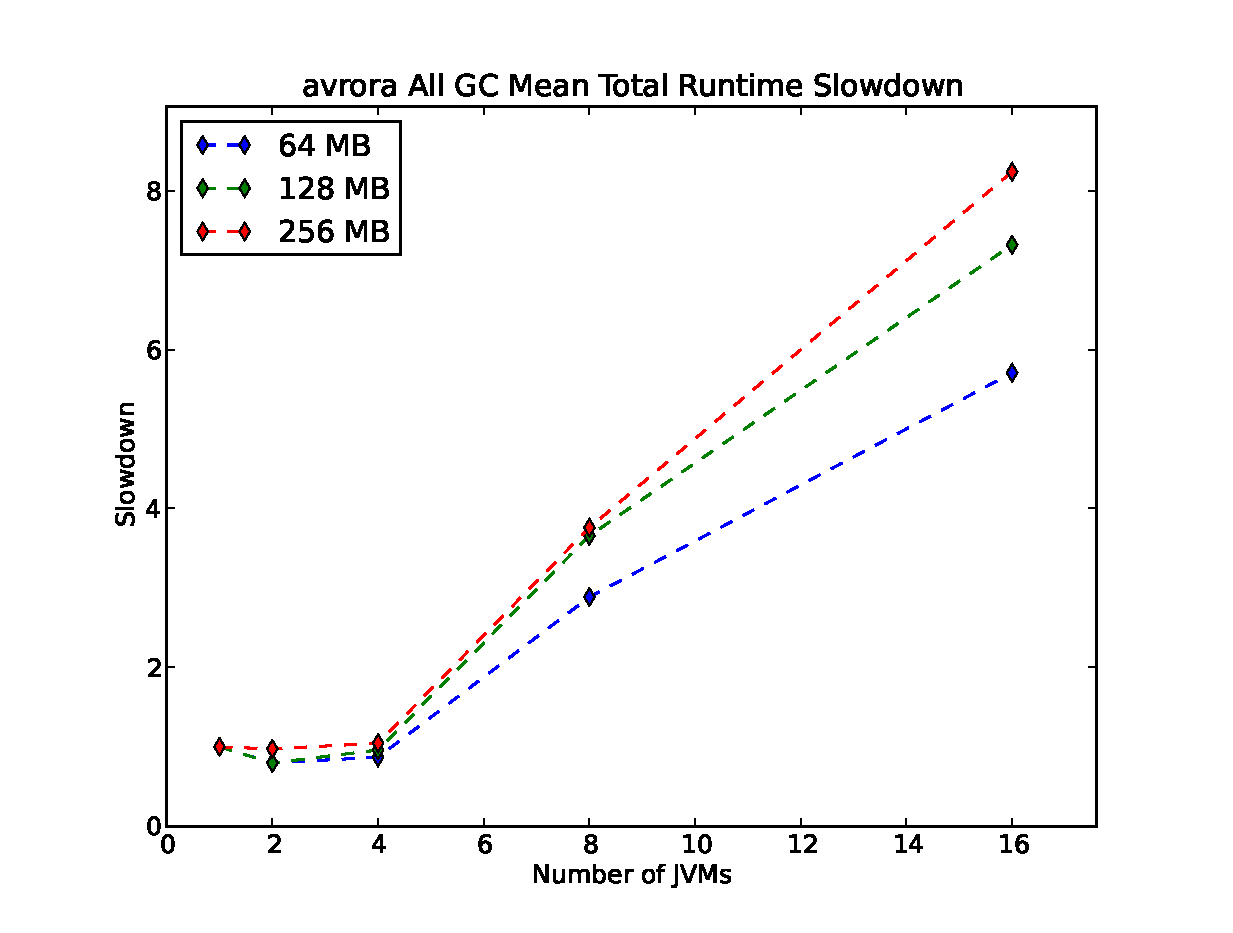
\epsfig{file=figures/gc/avrora.eps, height=2.3in, width=3.45in}
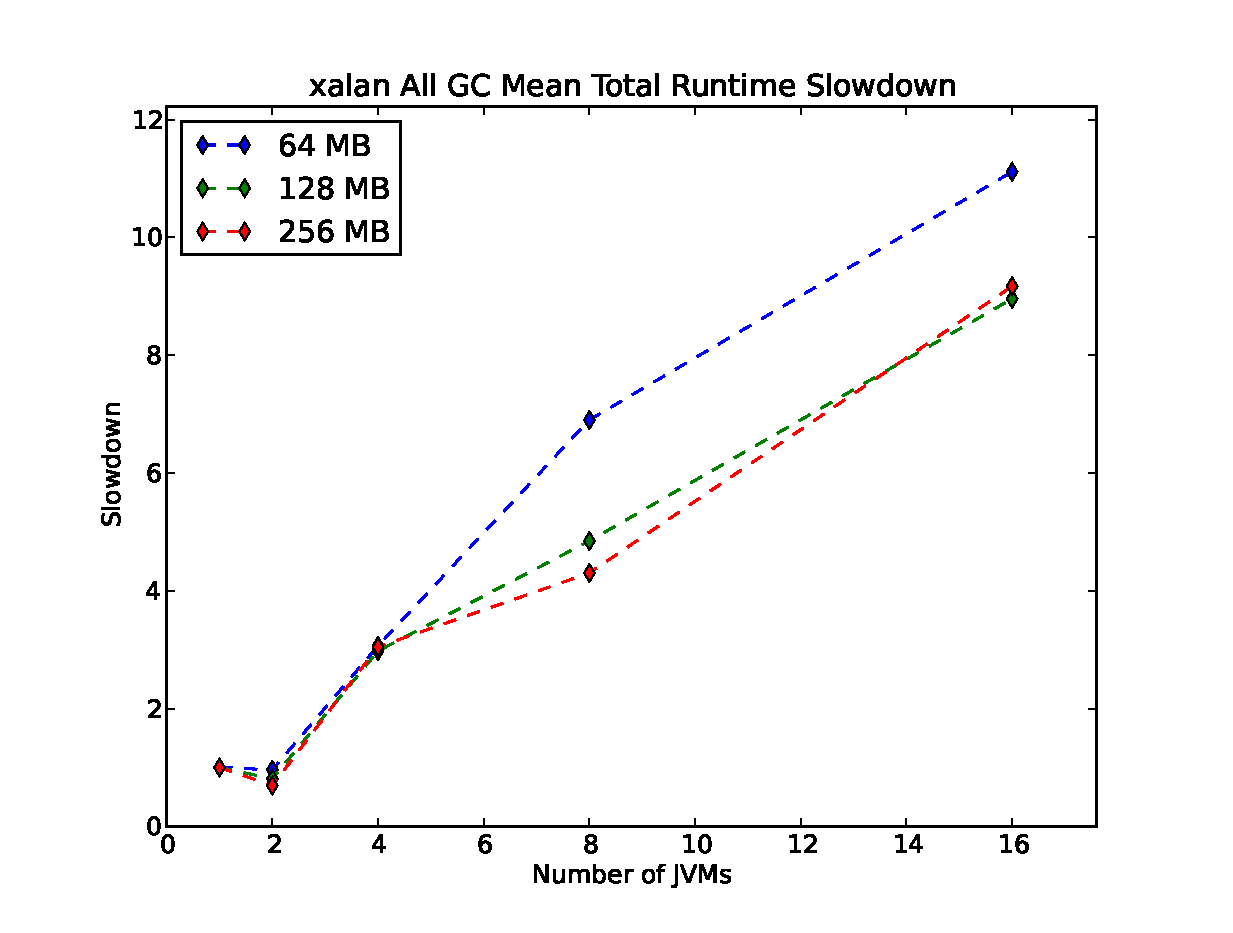
\epsfig{file=figures/gc/xalan.eps, height=2.3in, width=3.45in}
\caption{GC run time slowdown relative to 1 JVM.}
\label{fig:gcperf}
\end{figure*}

\subsubsection{Adaptive Optimizer Performance}
\begin{figure*}
\centering
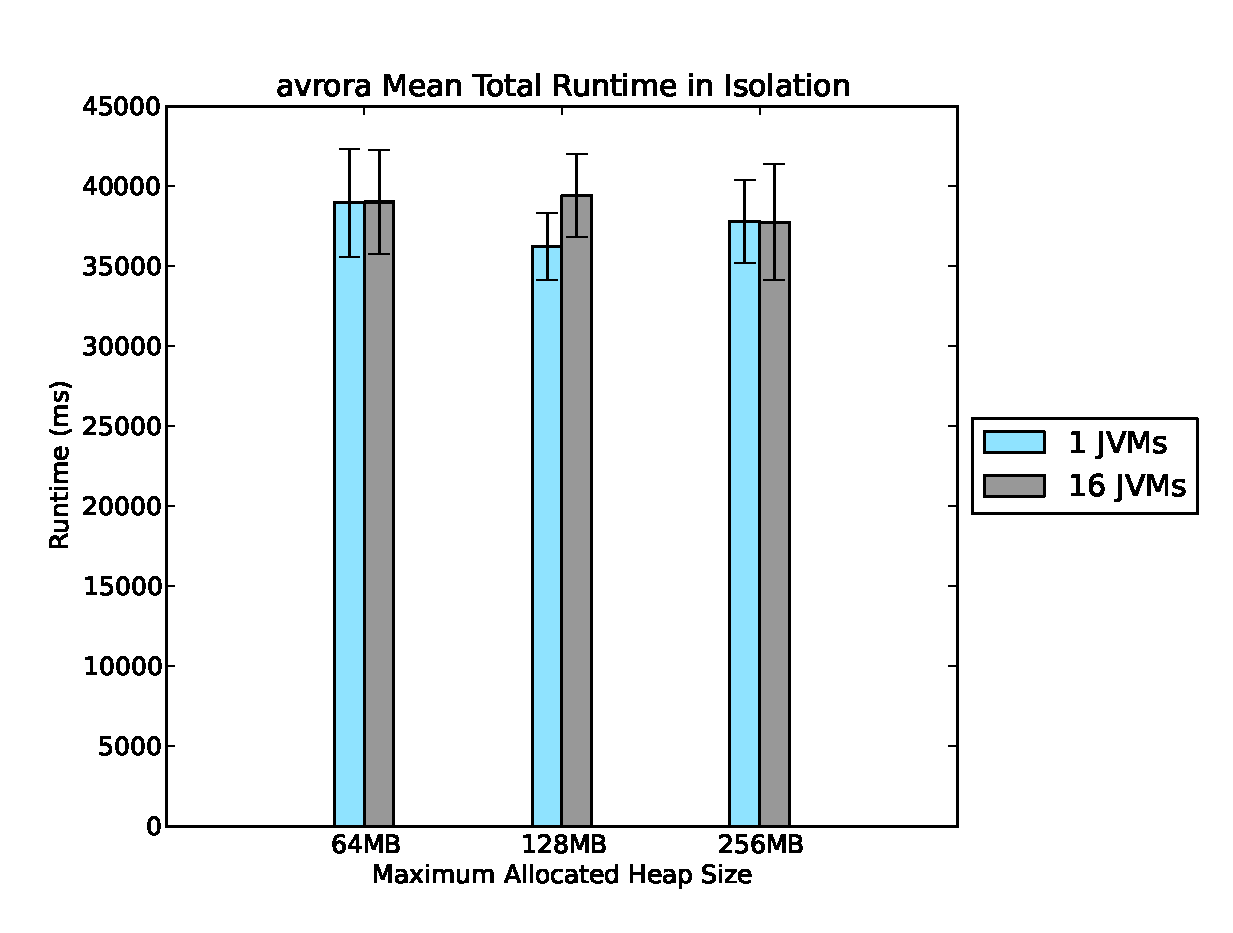
\epsfig{file=figures/jit/avrora.eps, height=2.3in, width=3.45in}
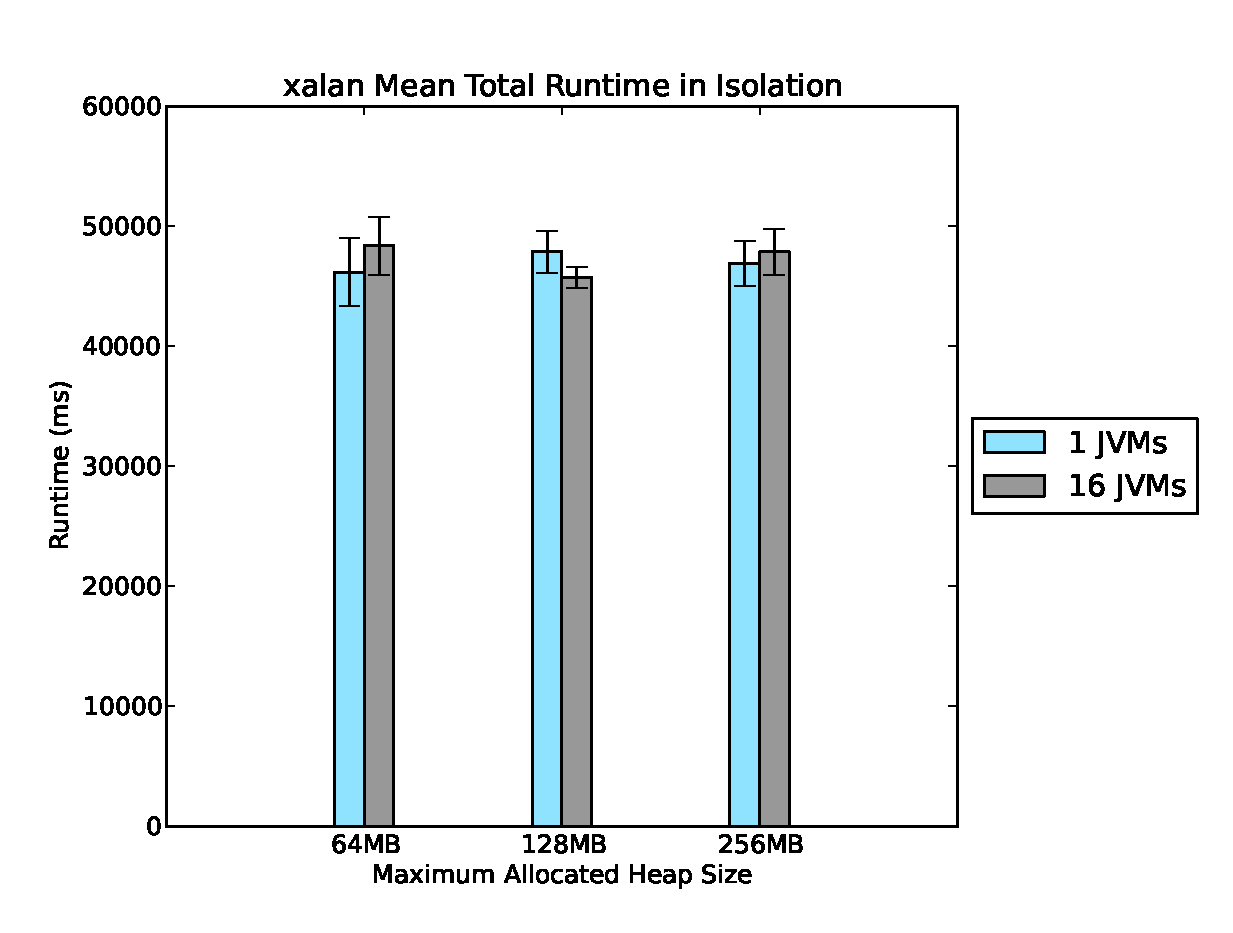
\epsfig{file=figures/jit/xalan.eps, height=2.3in, width=3.45in}
\caption{Mean total run time of JVMs warmed up in isolation and with 16 running JVMs in parallel.}
\label{fig:jitperf}
\end{figure*}
 
At run time, the HotSpot compiler performs extensive profiling of an application and uses that data to aggressively optimize machine code for the current execution environment \cite{hotspot:whitepaper}. We have demonstrated in section \ref{sssec:overallperfresults} that in the presence of multiple running JVMs, performance becomes more inconsistent for individual iterations. Thus, we hypothesize that if optimization occurs during a period of high load on the system, unpredictable performance may cause the adaptive optimizer to make \textit{poor decisions} translating the bytecode to optimal machine code for the system.

Figure~\ref{fig:jitperf} compares the performance of two different JVMs running a benchmark in isolation. Error bars of one standard deviation are displayed on the graph. We calculate the mean total running time of the next 5 iterations after warm up for 5 JVMs. For both avrora and xalan, there was no statistical difference between a JVM that has warmed up in isolation with a JVM that has warmed up with 15 other peers. The variation in iteration run times due to interference is not large enough to cause a JVM to optimize machine code differently. Any fine tuning of machine code is probably insignificant to performance compared to identifying and compiling hot spots in the first place. We do not expect the adaptive optimizer to benefit from gang scheduling.

\section{Cassandra with Xen} \label{sec:cassandra}

Cassandra is a write-optimized distributed NoSQL DBMS implemented in Java originally designed by Facebook \cite{lakshman2010cassandra}. It provides linear scalability and high availability, and the proven fault-tolerance on commodity hardware makes it a strong candidate for cloud infrastructure. As mentioned in seciton~\ref{sec:introduction}, Cassandra is now widely used on cloud computing side by popular tech companies like Twitter and Hulu \footnote{See http://planetcassandra.org/companies for a full list.}, running concurrently with other Java applications on a single machine. The experiment here attempts to investigate the interference and GC pressures that arise from running multiple Cassandra JVMs. This refers to some real world scenarios, such as Amazon Dynamo \cite{hastorun2007dynamo}, where multiple virtual nodes are running concurrently on a single physical node.

\subsection{YCSB}
To measure the performance of concurrent Cassandra instances, we use YCSB, Yahoo Cloud System Benchmark \cite{cooper2010benchmarking}, as our benchmark to issue workload requests to Cassandra nodes. It is also written in Java. With YCSB, we are able to control the request type and workload distribution. We also manage the total record size and request number to fit our machine capacity.

\subsection{Experimental Setup}
\begin{figure}
\centering
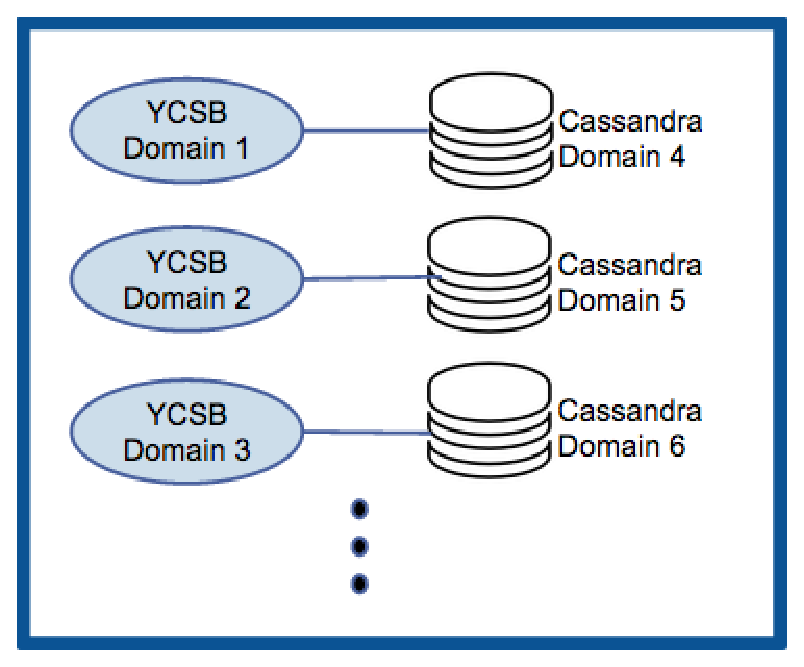
\epsfig{file=figures/cassandrasetupdigram.eps, height=2.25in, width=3in}
\caption{The set up of Cassandra and YCSB pairs}
\label{fig:cassandrasetup}
\end{figure}

\begin{figure*}

\centering
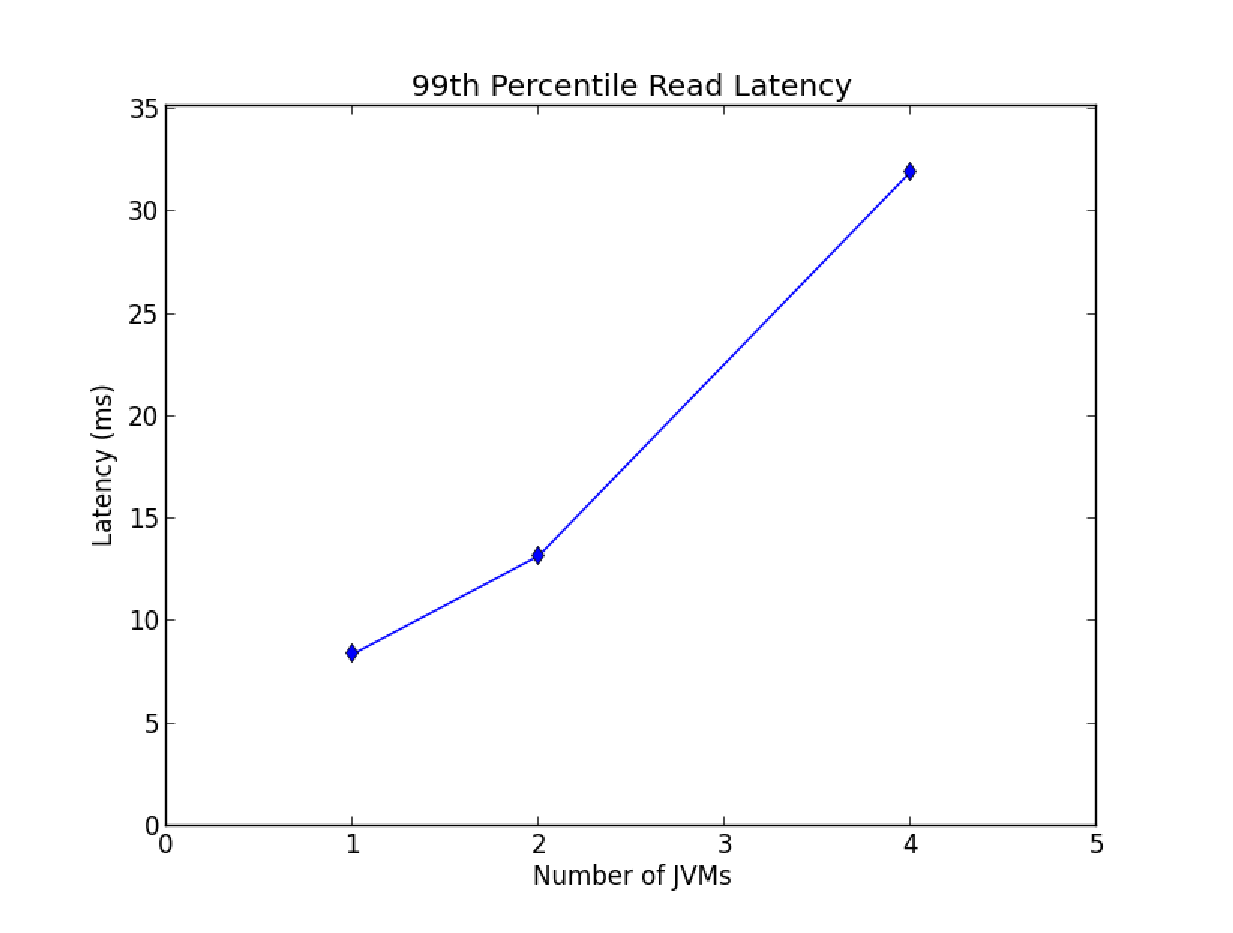
\epsfig{file=figures/cassandra/read99.eps,  height=1.5in, width=2.25in}
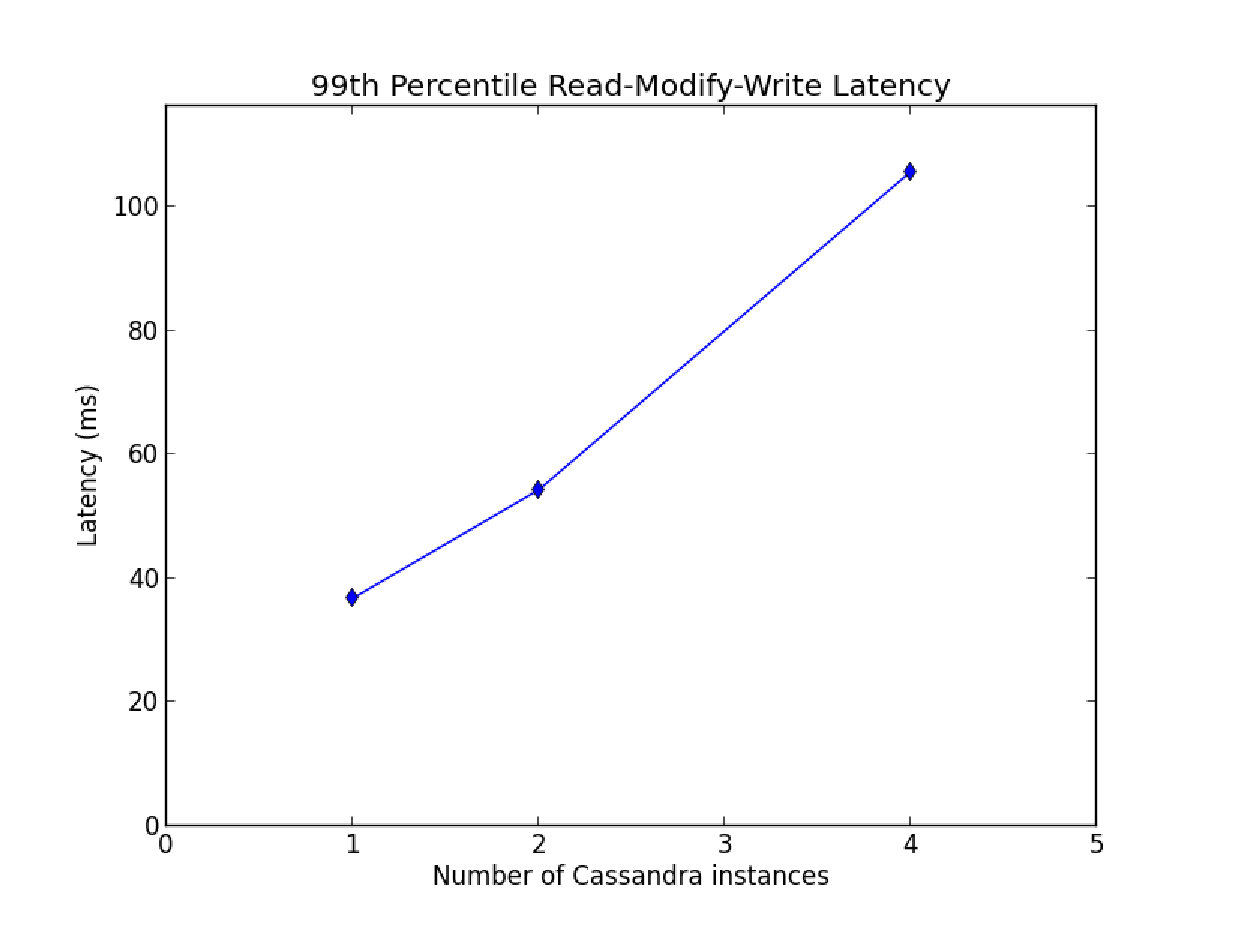
\epsfig{file=figures/cassandra/rw99.eps,  height=1.5in, width=2.25in}
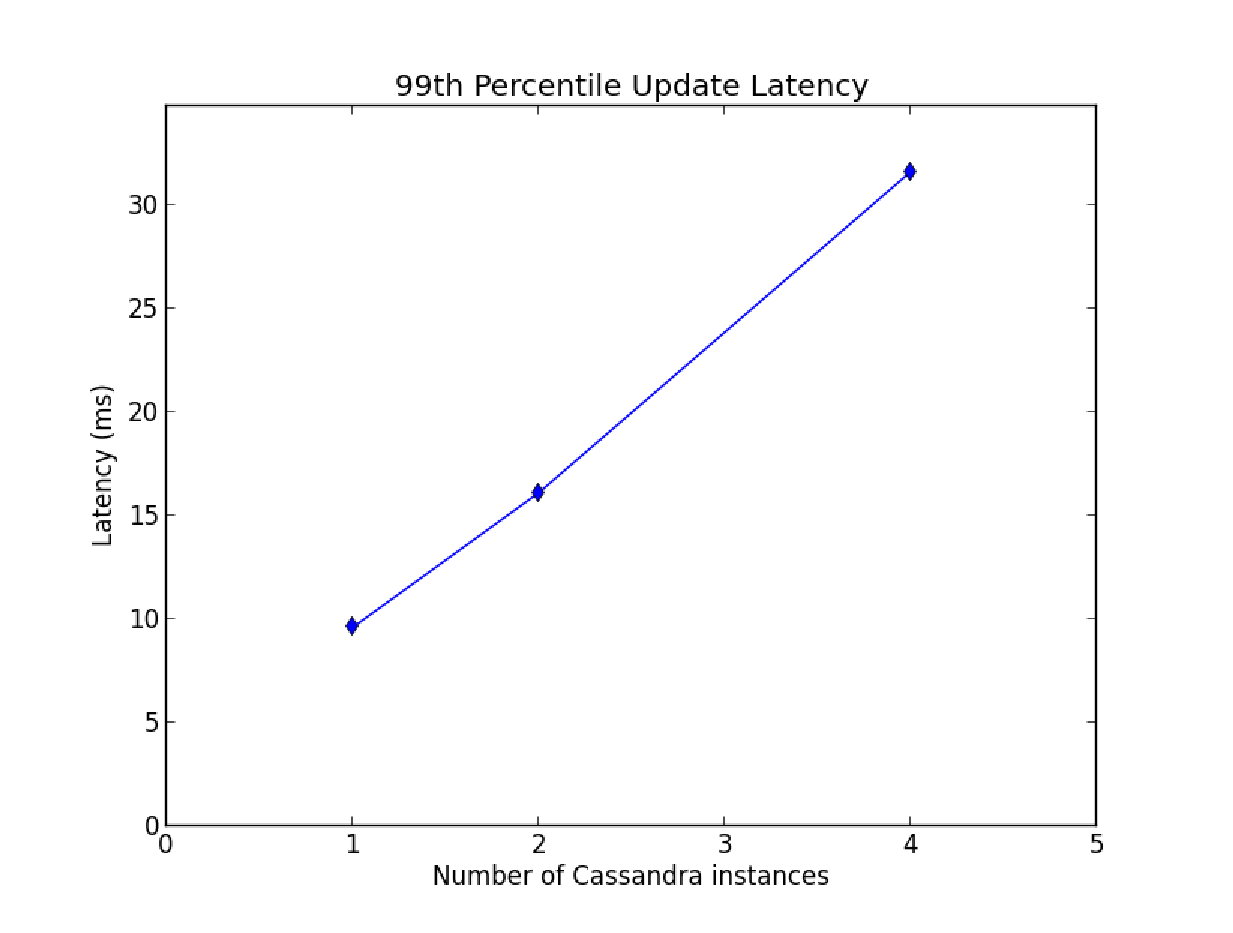
\epsfig{file=figures/cassandra/update99.eps,  height=1.5in, width=2.25in}
\caption{Operation-level 99 percentile latency increases as adding extra Cassandra instances for read, read-modify-write, and update.}
\label{fig:cassandraresults}
\end{figure*}

Our hardware setup for this experiment is identical to that in ~\ref{subsec:expsetup}. We run both Cassandra and YCSB as OS$^{v}$ guest domains upon Xen hypervisor on the same machine and infrastructure. Figure~\ref{fig:cassandrasetup} shows the architecture of our experiment. We pair each YCSB domain with one Cassandra domain to ensure that each Cassandra instance will receive the same number of requests and thereby maintain consistent workload across multiple Cassandra instances and eliminate load balancing as a potential source of variance. All domains are configured in a private LAN through a Xen bridge, to minimize the network influence on request latency and throughput. Given the high memory demand from Cassandra DBMS and the 12GB memory capacity of the test machine, we limit the memory allocation for each Cassandra and each YCSB domain to 2GB and 512MB respectively. This means we can scale up to at most 4 Cassandra plus 4 YCSB domains. All domains run with 6 virtual CPUs on the default Xen credit scheduler. Due to the above memory constraint, we cap the record count in each Cassandra database to 5000, with 10 fields each. The first field is the primary key, and the other 9 fields are of type \texttt{varchar}. We first measure the overall performance by benchmarking multiple Cassandra instances concurrently with two different types of workloads. We then measure the impact of increasing JVM count on the \textit{Concurrent-Mark-Sweep} garbage collector.

\subsubsection{Overall Performance}
Due to the memory limit, we only test with 1,2,4 cassandra instances, which involve 2,4,8 JVMs. We set the request count to 100,000 and run two kinds of workloads. The first one is update heavy, which consists of 50\% read and 50\% update. Typical application for this kind of workload is session store which records recent actions. The second workload involves a large portion of read-modify-write. Related applications include user database, where user records are read and modified by the user or to record user activity. This one has 50\% read and 50\% read-modify-write. Both workloads use zipfian distribution when picking record to update. This long-tail distribution, where the frequency of an item is inversely proportional to its rank, simulates the real world fact that a few records will be extremely popular while most records will be unpopular \cite{adamic2002zipf}. The data size is set to 1KB, so each field gets 100 bytes. For each benchmark, we first run a load phrase to populate the database, then run one iteration of run phrase to get Cassandra warm up. After that, we run 5 iterations of run phrase and record the overall as well as operation-level latency and throughput. The final value is measured as the average of those numbers across multiple JVMs during 5 iterations.

\subsubsection{Concurrent-Mark-Sweep Performance}
In the same setup as previous experiment, We run the Cassandra domains with flag \textit{-XX:+UseParNewGC} to turn on the \textit{CMS} collector. We record the GC time of both minor and major(mark and sweep) collection phrases during the execution of the 5 iterations of run phrase after warm up.

\begin{figure}
\centering
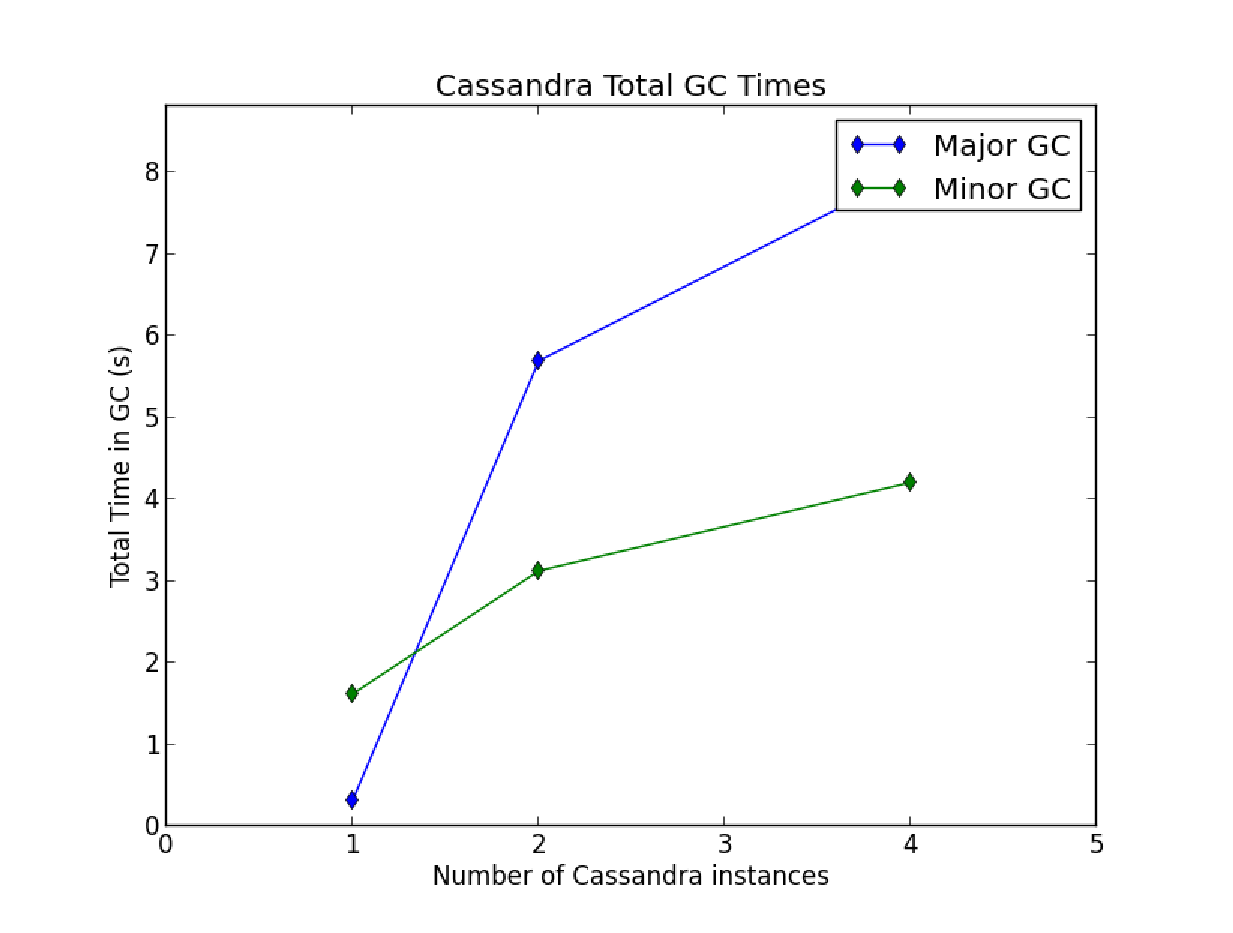
\epsfig{file=figures/cassandra/gc.eps, height=2.75in, width=3in}
\caption{GC total time increases under same workload with additional Cassandra instances}
\label{fig:cassandragc}
\end{figure}

\subsection{Results}
After running both workloads, we observed similar performance degradation relative to the number of Cassandra instances. Due to space limitations, we show the results of the read-modify-write workload here and hold them as representative.

\subsubsection{Overall Performance}
We showcase the individual 99$^{th}$ percentile latency plots for read, update, and read-modify-write operations in Figure~\ref{fig:cassandraresults}. The plots show  increases non-linearly from 1 to 2 to 4 ``pairs" of Cassandra-YCSB instances. When compared with writes, reads show a slightly larger degradation from 2 to 4 pairs than from 1 to 2 pairs. There is no saturation point as in the DaCapo experiment, and we expect that the robustness advantages of writes relative to reads is due to the write optimization of Cassandra, which utilizes \textit{memtable} and \textit{sstable} \cite{lakshman2010cassandra}. We hypothesize that the slowdown from 2 Cassandra-YCSB domains to 4 stems from the fact that in the 2 pair case, there are 4 JVMs in total, and all domains can be scheduled concurrently on 6 physical CPUs. However, with 4 domains and 8 total JVMs, not all domains can run at the same time. There is no guarantee that the scheduler would schedule the Cassandra instance and YCSB instance in each domain together. Thus, it is possible to have one side blocked while the other side is running. We discuss this issue further in section~\ref{sec:gs}.

\subsubsection{Concurrent-Mark-Sweep Performance}
Figure~\ref{fig:cassandragc} shows the increase of both major and minor GC time due to the additional Cassandra instances running. As the CMS collector uses the same parallel collector for the young generation from our DaCapo experiments, it is not surprising to see a pattern of minor GC slowdown identical to the one in section~\ref{sssec:overallperfresults}. We find the run time of minor GC increases linearly as a function of the number of concurrently running JVMs. This similarity confirms the early idea that synchronization between threads during garbage collection does not seem to be fine grained enough for scheduling interference to show a significant impact in our experiment.

\begin{figure*}
\centering
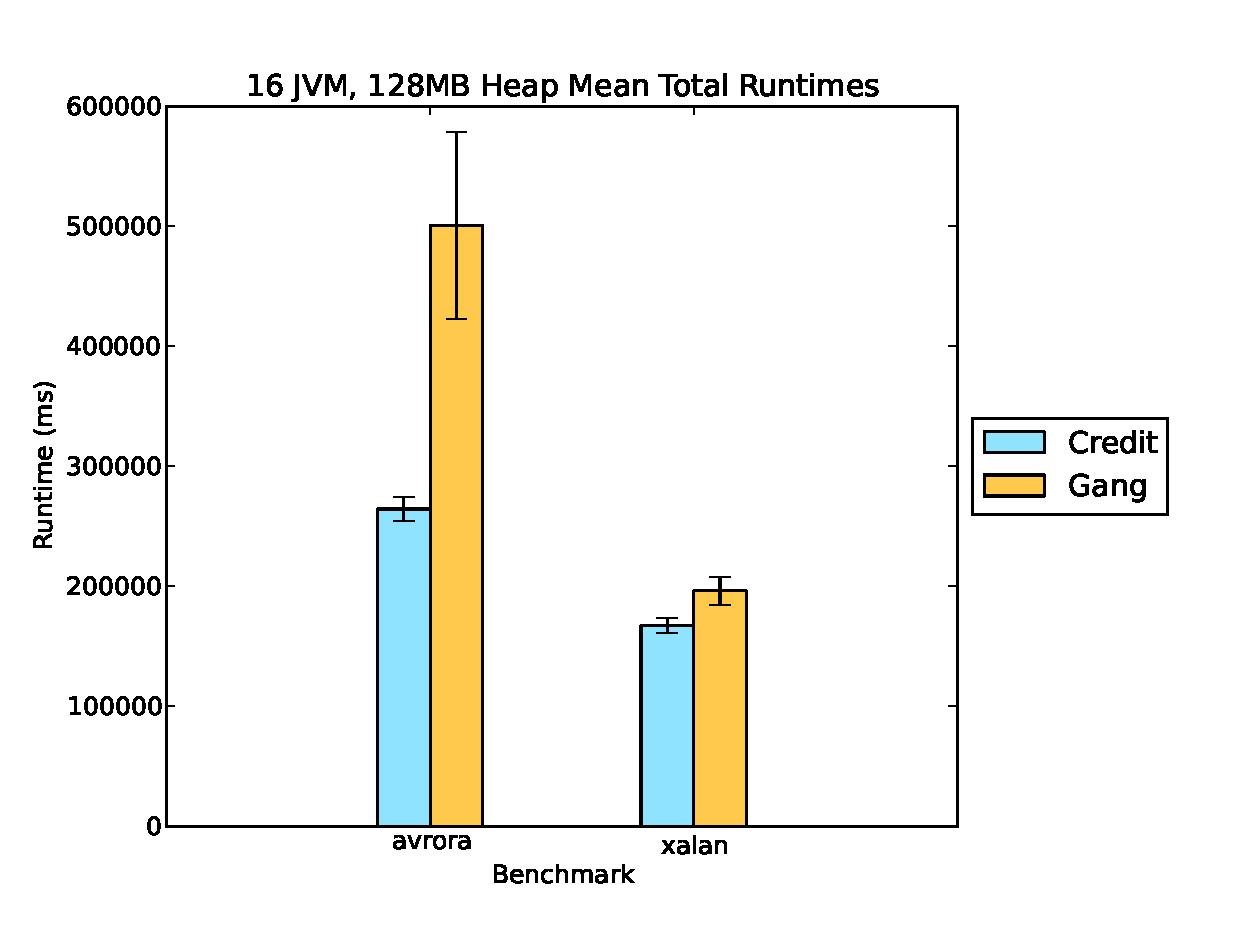
\epsfig{file=figures/gs/runtimes.eps, height=2.3in, width=3.45in}
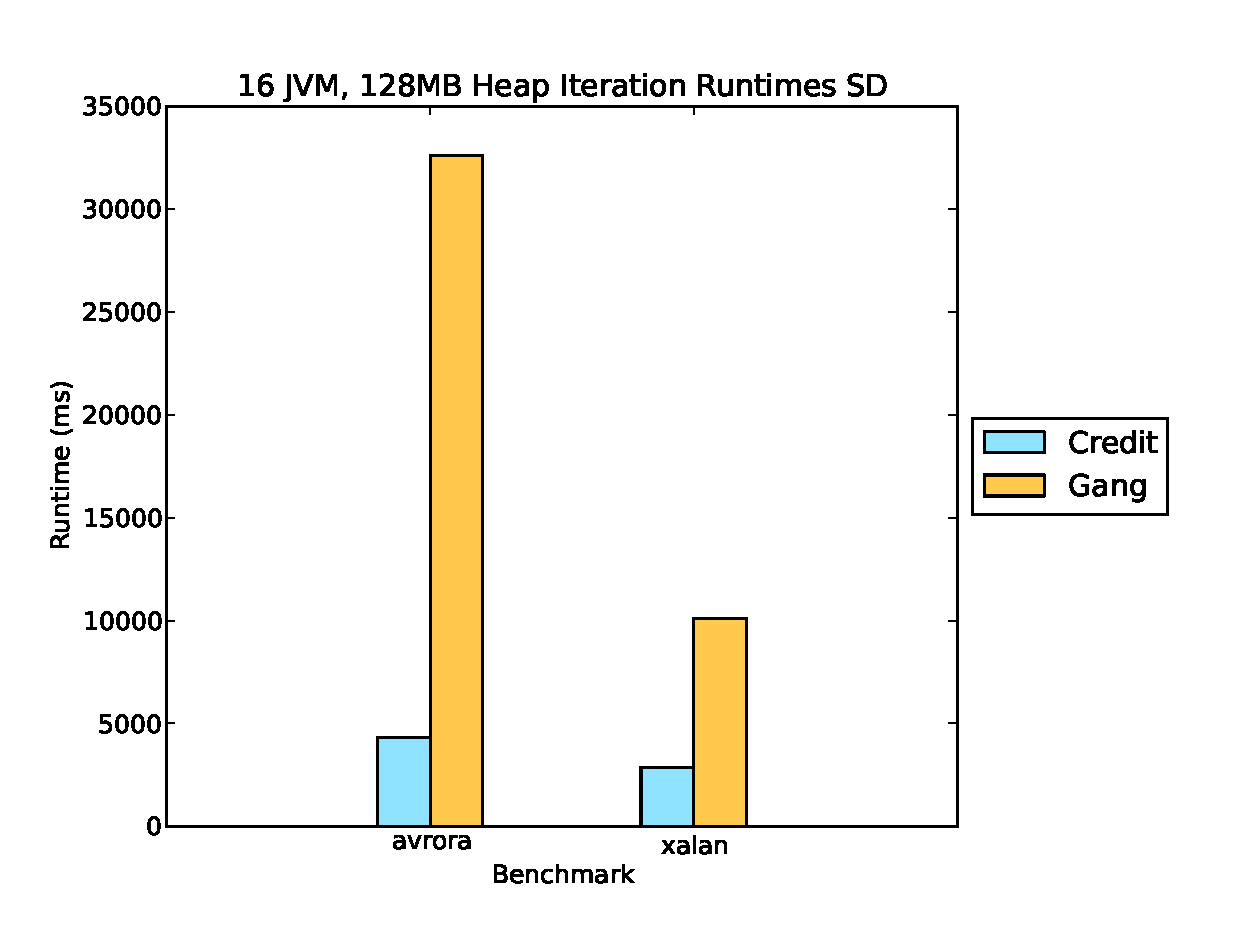
\epsfig{file=figures/gs/std.eps, height=2.3in, width=3.45in}
\caption{Overall performance and iteration standard deviation comparison of credit and gang scheduling}
\label{fig:gsresults}
\end{figure*}

\section{Gang Scheduling} \label{sec:gs}
A custom Xen hypervisor (Xen4Tess) featuring a prototype implementation of a gang scheduled CPU Pool was used for our gang scheduling experiments. The gang scheduler runs vCPUs of Xen domains one after another with a fixed 50ms scheduling quantum. Unfortunately, we were unable to install a stable version of Xen4Tess on our test machine. Furthermore, limitations in domains shutting down or doing anything other than running at full-boar prevented us from running our full experimental suite for both credit and gang scheduling in time. Before running an experiment with a new combination of benchmark and heap size, old running VMs are shutdown causing the whole machine to hang.

Nevertheless, we were able to get a similar setup to Figure~\ref{fig:dacaposetup} up and running on one our workstations to run small experiments on. In this setup a Xen4Tess hypervisor runs on a single-socket machine with an Intel Core i5-3570k processor at 3.4GHz (4 cores per socket, Hyperthreading off,  4 total CPUs) and 16GB of physical memory. Each Xen guest domain runs with 3 vCPUs and is allocated 512MB of memory. We run Xen domains within a 3-CPU Gang Scheduled Pool while reserving 1 CPU and 7GB of memory for Domain-0.

\subsection{Dacapo}
Using gang scheduling and this new machine, we reperformed the experiment in section \ref{sssec:overallperf} to measure overall performance for each of our benchmarks for only the 16 parallel JVMs, 128MB maximum heap size combination. However, we were unable to use xentrace and xenalyze to observe run states for gang scheduled domains because unexpected run state transitions would occur due to the gang scheduler.

Figure~\ref{fig:gsresults} shows the average overall total run time of avrora and xalan for both credit and gang scheduling. We graph the iteration run time standard deviations as well. In section~\ref{sssec:overallperf}, we hypothesized that overall performance will not improve much with gang scheduling. However, we did not expect that the gang scheduler would be so detrimental to performance. Avrora total run time increased 1.9x over credit scheduling while xalan increased 1.2x. When profiling the domain run states in section~\ref{sssec:overallperf}, we did discover that vCPUs block more often when scaling up to 16 JVMs. Because gang scheduling is unable to reassign pCPUs to different domains when the current domain's threads block, we end up wasting many CPU cycles that could be occupied with work from other domains. The over provisioning of CPU resources from gang scheduling also affects performance negatively because resource saturation does not occur until multiple JVMs are run in parallel.

We are surprised that run times for individual iterations become more unpredictable under the affects of gang scheduling, disproving our initial guess. We are unsure why this behavior is happening but perhaps there is large variation in how long vCPUs block for within a scheduling quantum. Blocking may occur early in the quantum, resulting in a lot of wasted CPU cycles, or not at all. Overall, gang scheduling does not benefit in any way that we could observe over the default credit scheduler for our DaCapo benchmarks.

\subsection{Cassandra} \label{subsec:cassandragang}
It is unfortunate that we could not get gang scheduling working on our test machine to repeat the previous Cassandra experiments, but some upcoming features of Xen4Tess and gang scheduling keep us believing that they would improve the test performance. We argue that gang scheduling could benefit final results on a couple of aspects \cite{feitelson1992gang}.
\\\textbf{I.} With gang scheduling, the system could schedule related threads or processes to run simultaneously on different processors. Take the previous Cassandra and YCSB experiment, the gang scheduler could be aware of their need to communicate and schedule them together. It avoids the situation that one side of communication is blocked while the other side is active.
\\\textbf{II.} A parallel job will achieve max overall progress if its components are evenly partitioned and execute simultaneously. Scheduling tasks in a gang run at same time and same pace helps threads to reach synchronization points at similar time. This applies to the scheduling of both major and minor GC threads in Cassandra experiments.

\section{Future Work} \label{sec:futurework}
As we are currently limited by the instability of Xen4Tess with gang scheduling on our test machine, we plan to replicate each of our DaCapo experiments with gang scheduling as soon as such a more stable implementation is available. This will enable us to more accurately compare benchmark behavior under gang scheduling with our base case.

We also plan to scale these experiments up on a machine with more resources and execute more JVM instances (32, 64, 100) to extract more evidence to verify our measurements. Similarly, we plan to also examine more types of workloads, including synthetic ones. We expect to find different results for workloads with finer grained synchronization and/or strict timing requirements. We wish to also run experiments using different combinations of garbage collection algorithms for young and old generations.

To verify our hypothesis in Section~\ref{subsec:cassandragang}, we plan to explicitly gang schedule processes which need mutual communication and experiment with more resource allocation policies. Besides that, we intend to explore the Tessellation event-triggered cell \cite{colmenares2013tessellation}, an ideal model for hosting services. It supplies a flexible event-handling as well as good responsiveness and resource utilization, which fit well with the role of Cassandra in our experiment.

\section{Related Work} \label{sec:relatedwork}
Our experiences with gang scheduling reflect some of the findings in \cite{peter2011technical}. In it, the authors describe how the benefits to gain from gang scheduling are not worth the complexity in implementing it for current workloads. The work asserts that a set of conditions, including latency sensitivity, fine-grained synchronization, burstiness, multiple high-priority workloads, must for gang scheduling to yield any significant benefits. However, it is possible an increasing number of future application workloads may fall into this category. We complement this work by evaluating how well the the combined workloads of Java applications and their associated JVMs fit and compare to such workloads. We describe our plans for evaluation of different workloads in section~\ref{sec:futurework}.

\textit{Callisto} is a resource management layer for parallel runtime systems. It utilizes dynamic spatial partitioning and co-scheduling in order to reduce the interference. The findings and accomplishments in Callisto is very similar to what we hope to achieve in this work. However, while Callisto targets general parallel runtime systems with CPU-intensive workloads, we focus specifically on JVM-specific tasks for applications with a wide variety of workloads.

Rather than strictly gang scheduling vCPUs together, the \textit{ESX} hypervisor by VMWare  uses a relaxed co-scheduling algorithm that ensures that the skew on each vCPU does not grow too large in comparison to its peers \cite{vmware:whitepaper}. vCPUs that are lagging behind can be run individually to catch up while those that advanced too far stop and wait. Although more overhead is needed to keep track of vCPU progress, the scheduler benefits by having more flexibility in scheduling choices.

\section{Conclusion} \label{sec:conclusion}
By utilizing a modified version of the Xen hypervisor that implements the Tessellation architecture, we provided baseline measurements on the performance of the DaCapo benchmarks and Cassandra's performance on the YCSB benchmark. We observed that for DaCapo, overall slowdown and GC overhead scaled linearly with increasing number of JVMs, but predictability in performance suffers. Multi-tenancy was also not detrimental to HotSpot's adaptive optimization. With Cassandra, we observed that 99\% latency measurements grow non-linearly with increasing number of JVMs. Unfortunately, due to  resource constraints, we were only able to extract a limited set of data points for this baseline. Thus, while we observed the trends above, we can not say with reasonable confidence they hold when scaling beyond 4 JVMs. Our measurements on a early-implementation of gang scheduled cells indicate that for the DaCapo benchmarks, performance drops significantly using the gang scheduler. Consistency in benchmark iteration run times surprisingly suffer as a result of gang scheduling as well. There are a number of possible explanations for this, including variance in time spent in blocked state and bugs in the implementation. Future work in exploring different Java applications and JVM components is needed to explore when gang scheduling may be beneficial for JVMs.


\section{Acknowledgments}
We would like to thank Martin Maas for advising us throughout our project along with Nathan Pemberton for writing the gang scheduler implementation for Xen, and Eric Roman and Kostadin Ilov for providing and setting up test machines.

% The following two commands are all you need in the
% initial runs of your .tex file to
% produce the bibliography for the citations in your paper.
\bibliographystyle{abbrv}
\bibliography{JVMTesselation}  % sigproc.bib is the name of the Bibliography in this case
% You must have a proper ".bib" file
%  and remember to run:
% latex bibtex latex latex
% to resolve all references
%
% ACM needs 'a single self-contained file'!
%

\balancecolumns
\end{document}
